% Code under BSD-3-Clause (see LICENSE). (c) 2026 Francesco Mario Antonio Mitrotta.
% Localised and spread softening damage in a strip pulled along its fibres, on a coarse and a fine mesh.
% (a) What the crack band assumes: one row of elements softens and the others unload, so breaking the
%     strip dissipates G per unit crack area on any mesh.
% (b) What can happen near the hole: every element of a zone of fixed size softens, so the energy grows
%     with the number of rows in the zone (3G on the coarse mesh, 6G on the fine one).
% Right: the softening law of one element in strain, eps_f = 2G/(sigma_0 L_c): halving L_c doubles eps_f,
%     so at the same strain the smaller element keeps more stress.
% Build: pdflatex 06_damage_localisation.tex
%        pdftocairo -png -r 200 -singlefile 06_damage_localisation.pdf 06_damage_localisation
\documentclass[tikz,border=4pt]{standalone}
\usetikzlibrary{arrows.meta,decorations.pathreplacing}
\begin{document}
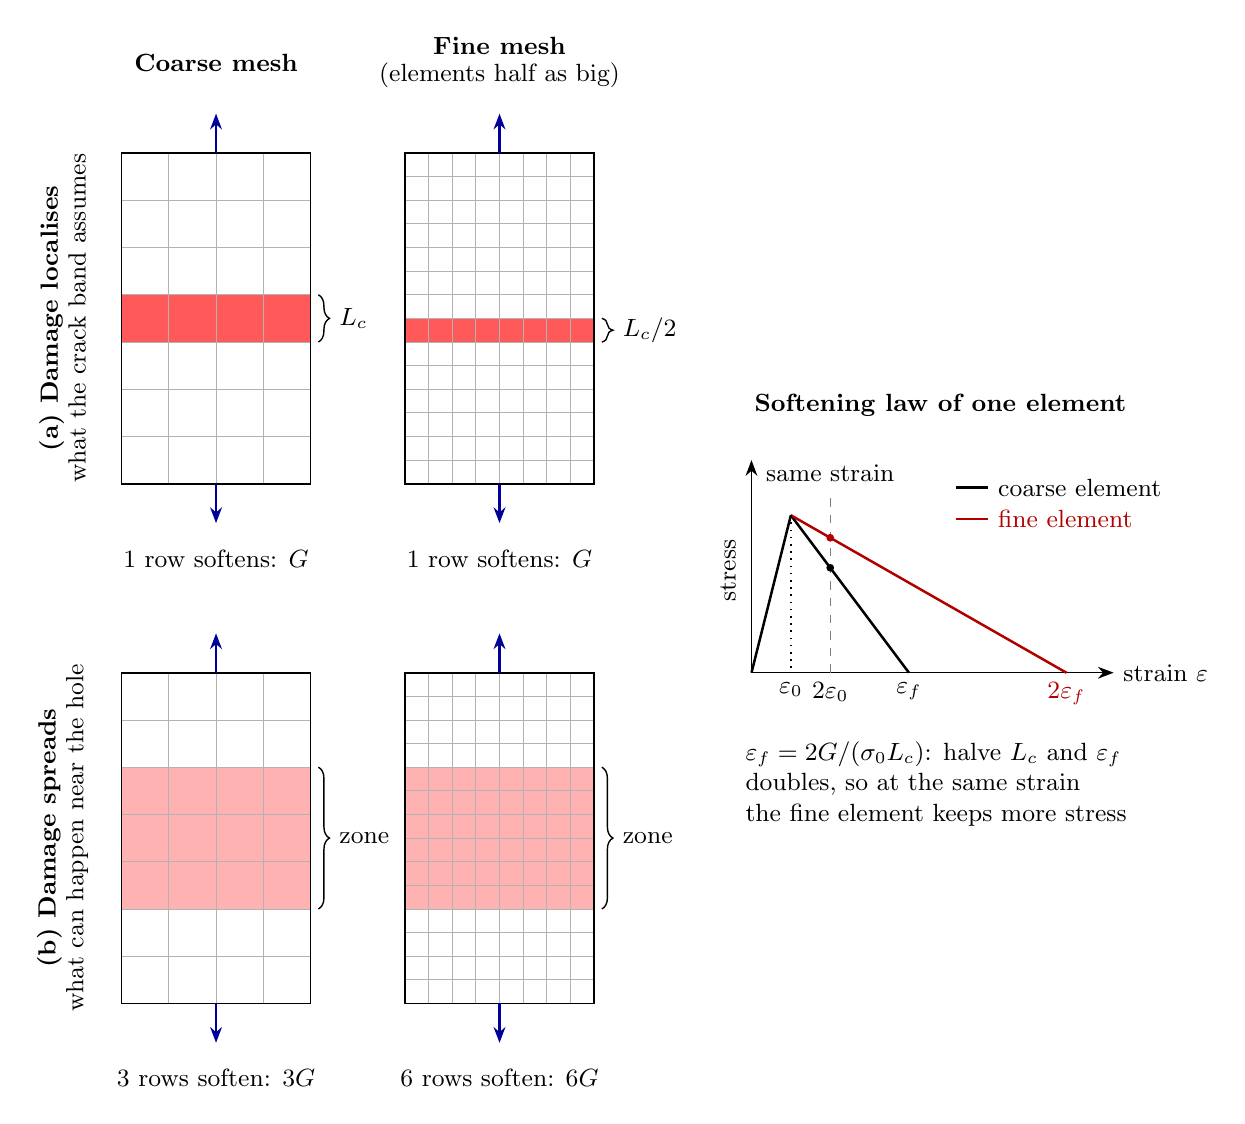
\begin{tikzpicture}[
    mesh/.style={draw=gray!60, line width=0.3pt},
    band/.style={fill=red!65},
    zone/.style={fill=red!30},
    load/.style={-{Stealth[length=2mm]}, line width=0.8pt, blue!60!black},
    lbl/.style={font=\small},
    head/.style={font=\bfseries\small},
    brace/.style={decorate, decoration={brace, amplitude=4pt}, line width=0.5pt},
  ]
  \def\W{2.4}   % strip width [cm]
  \def\H{4.2}   % strip height [cm]
  \def\Y{6.6}   % lower edge of the top row of strips [cm]
  % \strip{x}{y}{element size}{columns}{rows}: mesh of a W x H strip with its lower-left corner at (x, y),
  % drawn line by line (a TikZ grid with a step of 0.3 drifts by rounding), and the pull at both ends
  \newcommand{\strip}[5]{
    \foreach \i in {1,...,\numexpr#4-1\relax} \draw[mesh] (#1+\i*#3,#2) -- ++(0,\H);
    \foreach \j in {1,...,\numexpr#5-1\relax} \draw[mesh] (#1,#2+\j*#3) -- ++(\W,0);
    \draw[line width=0.6pt] (#1,#2) rectangle ++(\W,\H);
    \draw[load] (#1+\W/2,#2+\H) -- ++(0,0.5);
    \draw[load] (#1+\W/2,#2) -- ++(0,-0.5);
  }

  % ---------------- column and row headings ----------------
  \node[head] at (1.2,\Y+\H+1.15) {Coarse mesh};
  \node[head, align=center] at (4.8,\Y+\H+1.15) {Fine mesh\\[-1pt]\normalfont\small(elements half as big)};
  \node[head, rotate=90, align=center] at (-0.75,\Y+\H/2) {(a) Damage localises\\[-1pt]\normalfont\small what the crack band assumes};
  \node[head, rotate=90, align=center] at (-0.75,\H/2) {(b) Damage spreads\\[-1pt]\normalfont\small what can happen near the hole};

  % ---------------- (a) localised: one row softens, the rest unloads ----------------
  \fill[band] (0,\Y+1.8) rectangle ++(\W,0.6);          % one coarse row
  \strip{0}{\Y}{0.6}{4}{7}
  \draw[brace] (\W+0.1,\Y+2.4) -- (\W+0.1,\Y+1.8) node[midway, right=4pt, lbl] {$L_c$};
  \node[lbl] at (1.2,\Y-0.95) {1 row softens: $G$};

  \fill[band] (3.6,\Y+1.8) rectangle ++(\W,0.3);        % one fine row
  \strip{3.6}{\Y}{0.3}{8}{14}
  \draw[brace] (3.6+\W+0.1,\Y+2.1) -- (3.6+\W+0.1,\Y+1.8) node[midway, right=4pt, lbl] {$L_c/2$};
  \node[lbl] at (4.8,\Y-0.95) {1 row softens: $G$};

  % ---------------- (b) spread: every row of a fixed zone softens ----------------
  \fill[zone] (0,1.2) rectangle ++(\W,1.8);             % the same zone, 3 coarse rows
  \strip{0}{0}{0.6}{4}{7}
  \draw[brace] (\W+0.1,3.0) -- (\W+0.1,1.2) node[midway, right=4pt, lbl] {zone};
  \node[lbl] at (1.2,-0.95) {3 rows soften: $3G$};

  \fill[zone] (3.6,1.2) rectangle ++(\W,1.8);           % the same zone, 6 fine rows
  \strip{3.6}{0}{0.3}{8}{14}
  \draw[brace] (3.6+\W+0.1,3.0) -- (3.6+\W+0.1,1.2) node[midway, right=4pt, lbl] {zone};
  \node[lbl] at (4.8,-0.95) {6 rows soften: $6G$};

  % ---------------- the softening law of one element, in strain ----------------
  \begin{scope}[xshift=8.0cm, yshift=4.2cm]
    \draw[-{Stealth[length=2mm]}] (0,0) -- (4.6,0) node[right, lbl] {strain $\varepsilon$};
    \draw[-{Stealth[length=2mm]}] (0,0) -- (0,2.7);
    \node[lbl, rotate=90] at (-0.3,1.3) {stress};
    \draw[line width=0.9pt] (0,0) -- (0.5,2.0);                                   % elastic branch, the same for both
    \draw[line width=0.9pt, black] (0.5,2.0) -- (2.0,0);                          % coarse element: eps_f
    \draw[line width=0.9pt, red!70!black] (0.5,2.0) -- (4.0,0);                   % fine element: 2 eps_f
    \draw[dotted, line width=0.6pt] (0.5,2.0) -- (0.5,0) node[below, lbl] {$\varepsilon_0$};
    \node[below, lbl] at (2.0,0) {$\varepsilon_f$};
    \node[below, lbl, red!70!black] at (4.0,0) {$2\varepsilon_f$};
    \draw[dashed, gray] (1.0,0) -- (1.0,2.3) node[above, lbl, black] {same strain};
    \node[below, lbl] at (1.0,0) {$2\varepsilon_0$};
    \fill (1.0,1.333) circle (1.4pt);                                             % coarse: 1/3 of the stress lost
    \fill[red!70!black] (1.0,1.714) circle (1.4pt);                               % fine: 1/7 of the stress lost
    \draw[line width=0.9pt] (2.6,2.35) -- ++(0.4,0) node[right, lbl] {coarse element};      % legend
    \draw[line width=0.9pt, red!70!black] (2.6,1.95) -- ++(0.4,0) node[right, lbl, red!70!black] {fine element};
    \node[head] at (2.4,3.4) {Softening law of one element};
    \node[lbl, align=left, anchor=north west] at (-0.2,-0.75)
      {$\varepsilon_f = 2G/(\sigma_0 L_c)$: halve $L_c$ and $\varepsilon_f$\\doubles, so at the same strain\\the fine element keeps more stress};
  \end{scope}
\end{tikzpicture}
\end{document}
